\section{The Knowledge Base}
\label{sec:prelim}

To be able to understand the title of and the items in a top-$k$ page,
we need external, open-domain knowledge. In our work, we use
Probase~\cite{WuLWZ12:Probase}. In this section, we briefly introduce
Probase and how we use it to understand or ``conceptualize'' a short
piece of text.

Probase is a probabilistic knowledge base containing a large number
of concepts about worldly facts, which it acquires from billions of web
pages and years worth of search logs.  In Probase, a \emph{concept},
also known as a category may contain multiple \emph{instances},
and an \emph{instance} may also belong to multiple \emph{concepts}.
For example, ``fruit'' is a concept while ``apple'' and ``orange'' are
its instances.  Compared to other traditional knowledge bases, Probase
is distinctive in two aspects.  First, Probase has an extremely large
concept space. Currently it contains about 2.8 million concepts and 30
million instances.  Second, Probase is probabilistic in the sense that
for each relation, Probase provides conditional probabilities, also known as
\emph{typicality}, among other scores.  
For example, Probase scores how typical a ``robin'' and a
``penguin'' as instances of the ``bird'' concept. Such scores are
extremely important in text understanding.

We use Probase to understand a short piece of text through the
mechanism of ``conceptualization''.  Given a set of words or a short
text, the task is to derive one or multiple concepts that best match
the topic of the short text.  For example, given a word list
\{``India'',``China''\}, we may conceptualize it as ``Asian
countries''; then if we expand the list to
\{``India'',``China'',``Brazil''\}, the best match becomes ``BRIC
countries''.  Song et al. \cite{Song11:Conceptualize} proposed a
method of conceptualizing short text based on Probase using Naive
Bayes.  
%To evaluate their method, they conduct a series of experiments
%with thousands of tweets data, 
Results show that their system
outperforms all other existing approaches\cite{blei2003latent,wordnet,gabrilovich2006overcoming}.

\cut{%%%%%%%%%%%%%%% BEGIN CUT %%%%%%%%%%
In this section,
we will introduce several tools or concept which is key to our system,
including
DOM tree representation,
Conditional Random Field (CRF) \cite{CRFLafferty},
Stanford CoreNLP\cite{toutanova2003feature,finkel2005incorporating},
Probase\cite{WuLWZ12:Probase},
and short text conceptualization\cite{Song11:Conceptualize}.


%\subsection{DOM Tree Representation}
%\label{sec:DOMtree}
%In this paper, we focus on the list data of web pages, which are mostly written in HTML.
%\emph{The Document Object Model}, or DOM, presents an HTML page as a tree-structure, which is called DOM tree.
%This representation defines a standard way for accessing and manipulating HTML documents
%and is widely used in web information extraction and analysis.

%\emph{The Document Object Model (DOM)} defines
%a standard way for accessing and manipulating HTML documents
%and is widely used in web information extraction and analysis.
%It presents an HTML page as a tree-structure (DOM tree),
%and page elements as tag nodes in the tree.
%which has a tag name (like $<$strong$>$) and multiple attributes (like ``class'' and ``id'').
%The concept \emph{tag path} is the path from the root node to a certain tag node.
%For example, the tag path of the image tag in Figure \ref{fig:dotNet}(c) is
%``html/body/div/div/div/div/article/div/div/figure/img''.


%\begin{figure}[th]
%        \centering
%        \epsfig{file=./pics/DOMTree.eps,width=0.9\columnwidth}
%        \caption{A HTML sample page(a) and its corresponding DOM tree(b)}
%        \label{fig:DOMTree}
%\end{figure}
%
%Figure \ref{fig:DOMTree} shows a HTML fragment(a) as well as its corresponding DOM tree(b).
%As we can see in the figure, the nodes in the DOM tree have a hierarchical relationship to each other.
%Thus we follow the terms used in normal tree structure to describe the DOM tree, such as parent, child, root and leaf.
%In an HTML document, there are mainly three kinds of DOM tree nodes.
%
%\begin{itemize}
%  \item \textit{Tag node}:
%    A tag node represents an HTML element, such as a title or an image.
%    Each tag node has a tag name such as {\tt <h1>} or {\tt <p>}.
%    A tag node may contain one or more child nodes.
%    Usually a tag node has some attributes attached,
%    like the {\tt ``id'' } attribute of the {\tt h1} tag node in Figure \ref{fig:DOMTree}.
%  \item \textit{Text node}:
%    The texts in the HTML elements are contained in text nodes.
%    Since a text node cannot have children.
%    They should all be leaf nodes in the DOM tree.
%    Text nodes do not have a tag name or any attributes.
%  \item \textit{Comment node}:
%    Comment nodes contain comments in HTML documents.
%    They will not affect the actual rendering of an HTML page,
%    therefore our system ignores these nodes and filters them in the preprocessing step.
%\end{itemize}
%
%For every web page, the root node is {\tt <html> }.
%The {\tt <html> } node has two child nodes; {\tt <head> } and {\tt <body> }.
%{\tt <head> } node describes the properties and meta data of the document,
%including the title, scripts and external file link.
%{\tt <body> } node contains the main content of the document, including texts, links and images.
%For our system, we will first check the page title, which lies in the {\tt <title> } of the {\tt <head> } to see
%whether it is a potential top-$k$ page;
%then we will look into the {\tt <body> },trying to extract a list of nodes as result.

%Another important concept is the tag path.
%The tag path of a node is the path from that node to the root node.
%In our implementation,
%we use a string that concatenate the tag names of the nodes in order
%to represent a tag path.
%Since the text nodes do not have a tag name, we manually name them as {\tt <text>}.
%Table \ref{tab:tagpath} shows all the tag paths in the HTML fragment (Figure \ref{fig:DOMTree}(a)).
%
%\begin{table}
%\centering
%\caption{The tag paths in Figure \ref{fig:DOMTree}(a)}
%\begin{tabular}{|l|} \hline
%html\\
%html/head\\
%html/head/title\\
%html/head/title/text\\
%html/body\\
%html/body/h1\\
%html/body/h1/text\\
%html/body/p\\
%html/body/p/text\\
%\hline
%\end{tabular}
%\label{tab:tagpath}
%\end{table}
%


%\subsection{Conditional Random Field (CRF)}
%
%\label{sec:crf}

\emph{Conditional Random Field}, or CRF\cite{CRFLafferty},
is a probabilistic model based on undirected graphs.
It is used to encode known relationships between observations and construct consistent interpretations.
%Recently, CRF is widely used in natural language processing.
%Applications include part of speech tagging, shallow parsing,
%name entity recognition and so on,
%all of which have obtained satisfying results.
%CRF is one of the most popular method in machine learning.
The main idea of CRF is to calculate the conditional probability
of the whole label sequence given the observation sequence.
If we define $X(X_{1},X_{2},X_{3},...,X_{n})$ as observations
(the data sequence to label), and $Y(Y_{1},Y_{2},Y_{3},...,Y_{n})$
as random variables (any possible label sequence),
CRF needs to calculate the conditional distribution $P(Y|X)$,
and then select the $Y$ that maximize the probability.
We can build an undirected graph $G(V,E)$ to represent each $Y_{i} \in Y$
according to the independency relations
(in other words, if $Y_{i}$ and $Y_{j}$ depend on each other,
there is an edge connecting the two nodes).
Therefore, the overall probability $P(Y|X)$ is equal to
the product of the potential functions of all the maximal cliques in $G(V,E)$.
%In our system, we use CRF++, which is a simple,
%customizable and open source implementation written in C++.

%As mentioned in \ref{sec:intro}, before we extract top-$k$ list from a web page,
%we must make sure the page is a top-$k$ list. We do this by analyzing the title of the page,
%in other words, we build a classifier for the page titles.
%At the heart of this classifier, Conditional Random Field is used for model training and learning.
%
%Conditional Random Field, or CRF\cite{CRFLafferty}, is a probabilistic model based on undirected graphs. It is used to encode known relationships between observations and construct consistent interpretations. Recently, CRF is widely used in natural language processing. Applications include part of speech tagging, shallow parsing, name entity recognition and so on, all of which have obtained satisfying results. CRF is one of the most popular method in machine learning.
%
%The main idea of CRF is to calculate the conditional probability of the whole label sequence given the observation sequence.
%The structure of the label sequence can be an arbitrary undirected graph, which is different from hidden Markov model\cite{HMMBaum}.
%Since in normal NLP tasks (including the title classifier in our system), the graph of interest is usually a linear chain. We will focus on this model in the following discussion.
%
%If we define $X(X_{1},X_{2},X_{3},...,X_{n})$ as observations (the data sequence to label), and $Y(Y_{1},Y_{2},Y_{3},...,Y_{n})$ as random variables (any possible label sequence), CRF needs to calculate the conditional distribution $P(Y|X)$, and then select the $Y$ that maximize the probability. We can build an undirected graph $G(V,E)$ to represent each $Y_{i} \in Y$ according to the independency relations (in other words, if $Y_{i}$ and $Y_{j}$ depend on each other, there is an edge connecting the two nodes).
%Therefore, the overall probability $P(Y|X)$ is equal to the product of the potential functions of all the maximal cliques in $G(V,E)$.
%Since in a linear chain, only the adjacent two nodes can form a cliques, $P(Y|X)$ can be expressed as a product of $P(Y_{i}|X),P(Y_{i},Y_{i-1}|X)$.
%
%According to the definition of the exponential probabilistic model and Conditional Random Field, for a linear chain graph $G(V,E)$,
%$P(Y|X)$ can be normalized by the following equation:
%\begin{equation}\label{equ:crf1}
%    P(Y|X)=\exp(\sum_{j}\lambda_{j}t_{j}(y_{i-1},y_{i},x,i)+\sum_{k}\mu_{k}s_{k}(y_{i},x,i))
%\end{equation}
%
%In this equation, $\sum_{j}\lambda_{j}t_{j}(y_{i-1},y_{i},x,i)$ is the function corresponding to $P(Y_{i},Y_{i-1}|X)$ ,
% $\sum_{k}\mu_{k}s_{k}(y_{i},x,i))$ is the function corresponding to $P(Y_{i}|X)$, $t_{j}$ and $s_{k}$ are feature functions, while
%$\lambda_{j}$ and $\mu_{k}$ are parameters to be estimated from training data.
%
%When defining feature functions, we construct a set of real-valued features of the observation to express some characteristic of the empirical distribution of the training data. Each feature function is related to one or multiple features. When the features are satisfied, the function value will be $1$ (otherwise it will be $0$).
%
%Since $s_{k}(y_{i},x,i)$ can be written as $s_{k}(y_{i-1},y_{i},x,i)$, we can put $t_{j}$ and $s_{k}$ in the same form: $f_{k}(y_{i-1},y_{i},x,i)$.
%Therefore, Equation \ref{equ:crf1} can be simplified as
%
%\begin{equation}\label{equ:crf2}
%    P(Y|X)=\frac{1}{Z(x)}\exp(\sum_{j}\lambda_{j}F_{j}(y,x))
%\end{equation}
%where $F_{j}(y,x)=\sum_{i=1}^{n}f_{j}(y_{i-1},y_{i},x,i)$ and $Z(x)$ is a normalization factor.
%With training data (a set of labeled data sequence ${(x^{(k)},y^{(k)})}$),
%we can infer parameters $\lambda_{j}$ through
%maximum likelihood learning algorithm.
%
%For further details on CRF,
%you can refer to this list\cite{CRFLafferty,wallach2004conditional,sutton2006introduction}.
%
%There are many implementation of CRF. In our system, we use CRF++,
%which is a simple, customizable and open source implementation written in C++. CRF++ is designed for generic purpose and shows its power in a variety of NLP tasks, such as Named Entity Recognition, Information Extraction and Text Chunking.
%

%\subsection{Stanford Parser}
%\label{sec:stanfordParser}
%
\emph{Stanford CoreNLP} is an integration of
several state-of-art natural language analysis tools
including a part-of-speech tagger\cite{toutanova2003feature},
a parser\cite{StanfordParser},
a named-entity recognizer \cite{finkel2005incorporating} and so on.
It provides the foundational building blocks for higher level text understanding applications.
}%%%%%%%%%%%%%%%% END OF CUT %%%%%%%%%%%%%%

%which are competent for most NLP tasks such as
%part-of-speech tagging, named-entity recognition,
%deep parsing and so on.
%It provides the foundational building blocks for higher level text understanding applications.
%Among these tools, \emph{Stanford Part-Of-Speech Tagger}
%\cite{toutanova2003feature} and \emph{Stanford Named Entity Recognizer }
%\cite{finkel2005incorporating} are utilized in our system.
%The former is a maximum-entropy (CMM) tagger for English words,
%using the Penn Treebank tag set \cite{marcus1993building}.
%While the latter uses a Conditional Random Field sequence model,
%together with well-engineered features for Named Entity Recognition in English,
%which enables us to detect and normalize date and location information in titles.


%As mentioned in Subsection \ref{sec:crf}, we use CRF to generate the title classifier model.
%To enhance the accuracy of the model, some lexical and semantic features are applied,
%such as part of speech (POS tag), lemma and so on.
%In order to automatically generate these features for both training and test data,
%we need the help of a natural language processing tool,
%which is the Stanford Parser in our system.
%
%Stanford Parser is an open-source natural language parser that is written in Java.
%It contains both an unlexicalized parser and a lexicalized one,
%and the former one is of our interest.
%The unlexicalized parser is based on optimized probabilistic context free grammar(PCFG) and lexicalized syntax dependency.
%The probabilistic model is used to select the best, in other words, the most likely one from multiple parsing results of the input sentence,
%while the lexicalized dependency indicates the dependency information among each component of the sentence.
%The parser learns knowledge of language from Penn treebank\cite{marcus1993building}
%which contains a large number of hand-parsed sentences.
%
%As we can see in Figure \ref{fig:parserRes},
%the output of Stanford Parser can be in various formats,
%which we listed as follows:
%
%\begin{figure}[th]
%        \centering
%        \epsfig{file=./pics/parserRes.eps,width=0.6\columnwidth}
%        \caption{Stanford Parser: a sample query(a) and results(b-d)}
%        \label{fig:parserRes}
%\end{figure}
%
%\begin{itemize}
%  \item \textit{POS tagging}:
%  As is shown in Figure \ref{fig:parserRes}(b), the parser can offer the part of speech for each word.
%  Stanford Parser follows The Penn Treebank Tag Set \cite{PennTreeBankTagSet}, which is listed in Table \ref{tab:tagSet}.
%  \item \textit{Lemma}:
%  Lemma indicates the original form of the word, like the singular form of a plural noun or
%  the base form of a past participle. For example, in the query in Figure \ref{fig:parserRes}(a), the lemma for ``best'' is ``good'',
%  while the lemma for ``players'' is ``player''.
%  \item \textit{Parse}:
%  In this format, the parser gives the phrase structure tree,which shows the hierarchy of the query sentence.
%  For instance, in Figure \ref{fig:parserRes}(d), the phrase ``one of the best NBA players'' is treated as a ``NP''(noun phase) as a whole,
%  which is also the child of the verb ``is''.
%  \item \textit{Typed dependency representation}:
%  This format will present a set of Stanford dependencies, from which we can analyze the head word based on the phrase structure.
%  In Figure \ref{fig:parserRes}(c), each line is a typed dependency.
%  For example, the 8th dependency is noun compound modifier, that a noun (``NBA'', word No. 8) serves to modify the head noun(``players'', word No.9).
%\end{itemize}
%
%\begin{table}
%\centering
%\caption{The Penn Treebank Tag Set \cite{PennTreeBankTagSet}}
%\begin{tabular}{|l|l|l|} \hline
%\textbf{Number}	&\textbf{Tag}	&\textbf{Description}\\ \hline
%1. 	&CC 	&Coordinating conjunction\\
%2. 	&CD 	&Cardinal number\\
%3. 	&DT 	&Determiner\\
%4. 	&EX 	&Existential there\\
%5. 	&FW 	&Foreign word\\
%6. 	&IN 	&Preposition or subordinating conjunction\\
%7. 	&JJ 	&Adjective\\
%8. 	&JJR 	&Adjective, comparative\\
%9. 	&JJS 	&Adjective, superlative\\
%10. 	&LS 	&List item marker\\
%11. 	&MD 	&Modal\\
%12. 	&NN 	&Noun, singular or mass\\
%13. 	&NNS 	&Noun, plural\\
%14. 	&NNP 	&Proper noun, singular\\
%15. 	&NNPS 	&Proper noun, plural\\
%16. 	&PDT 	&Predeterminer\\
%17. 	&POS 	&Possessive ending\\
%18. 	&PRP 	&Personal pronoun\\
%19. 	&PRP\$ 	&Possessive pronoun\\
%20. 	&RB 	&Adverb\\
%21. 	&RBR 	&Adverb, comparative\\
%22. 	&RBS 	&Adverb, superlative\\
%23. 	&RP 	&Particle\\
%24. 	&SYM 	&Symbol\\
%25. 	&TO 	&to\\
%26. 	&UH 	&Interjection\\
%27. 	&VB 	&Verb, base form\\
%28. 	&VBD 	&Verb, past tense\\
%29. 	&VBG 	&Verb, gerund or present participle\\
%30. 	&VBN 	&Verb, past participle\\
%31. 	&VBP 	&Verb, non-3rd person singular present\\
%32. 	&VBZ 	&Verb, 3rd person singular present\\
%33. 	&WDT 	&Wh-determiner\\
%34. 	&WP 	&Wh-pronoun\\
%35. 	&WP\$ 	&Possessive wh-pronoun\\
%36. 	&WRB 	&Wh-adverb \\
%\hline
%\end{tabular}
%
%\label{tab:tagSet}
%\end{table}



